\subsection{Dãy graphic}

% \begin{tcolorbox}[breakable]
%     \begin{baitoan}[\parencite{shahriari2021invitation}, P10.1.13, p. 368]\label{pb:w02:08}
%         ~
        
%         \begin{enumerate}
%             \item[(a)] Chứng minh rằng nếu dãy $d_1,\,d_2,\,\ldots,\,d_p$ là một dãy graphic khi và chỉ khi dãy $p - d_p - 1,\,\ldots,\,p-d_2-1,\,p-d_1-1$ cũng là một dãy graphic.
%             \item[(b)] Hỏi dãy $9,\,9,\,9,\,9,\,9,\,9,\,9,\,9,\,8,\,8,\,8$ có phải là một dãy graphic không? 
%         \end{enumerate}
%     \end{baitoan}
% \end{tcolorbox}

% \textbf{Lời giải. }

\begin{enumerate}
    \item[(a)] Xét đồ thị đơn với dãy bậc $d_1,\,d_2,\,\ldots,\,d_p$, ta thêm vào các cạnh để trở thành đồ thị đầy đủ và bỏ đi những cạnh ban đầu. Khi đó đồ thị thu được là đồ thị với dãy bậc $p - d_p - 1,\,\ldots,\,p-d_2-1,\,p-d_1-1$ nên ta có điều phải chứng minh.
    \item[(b)] Áp dụng tính chất ở ý (a), dãy $9,\,9,\,9,\,9,\,9,\,9,\,9,\,9,\,8,\,8,\,8$ là một dãy graphic khi và chỉ khi dãy $2,\,2,\,2,\,1,\,1,\,1,\,1,\,1,\,1,\,1,\,1$ là một dãy graphic. Theo thuật toán Havel-Hakimi, điều đó tương đương với $1,\,1,\,1,\,1,\,1,\,1,\,1,\,1,\,1,\,1$ cũng là một dãy graphic; điều này đúng vì tồn tại đồ thị có dãy bậc là dãy này, chẳng hạn xét đồ thị 10 đỉnh trong đó các đỉnh được chia thành 5 cặp, mỗi đỉnh trong một cặp nối với nhau (hay nói cách khác là 5 đoạn thẳng rời nhau).
\end{enumerate}

\begin{tcolorbox}[breakable]
    \begin{baitoan}[\parencite{shahriari2021invitation}, P10.1.14, p. 368]\label{pb:w02:07}
        Xét đồ thị đơn 6 đỉnh có bậc của năm đỉnh lần lượt là 5, 4, 4, 2, 2. Hỏi bậc của đỉnh thứ sáu có thể nhận những giá trị nào?
    \end{baitoan}
\end{tcolorbox}

\textbf{Lời giải. }Theo định lý Euler, bậc của đỉnh còn lại phải là số lẻ, nên phải thuộc $\{1,\,3,\,5\}$. 

\textbf{Trường hợp 1. }Bậc của đỉnh còn lại bằng 5. Khi đó, dãy bậc của đồ thị là $5,\,5,\,4,\,4,\,2,\,2$, là một dãy graphic. Theo thuật toán Havel-Hakimi, dãy $4,\,3,\,3,\,1,\,1$ và $2,\,2,\,0,\,0$ cũng là các dãy graphic. Tuy nhiên, không tồn tại đồ thị đơn 4 đỉnh có dãy bậc là $2,\,2,\,0,\,0$; vì có hai đỉnh không nối với đỉnh nào, nên trong hai đỉnh còn lại chỉ có thể có bậc cao nhất bằng 1. Do đó bậc của đỉnh còn lại của đồ thị đã cho không thể bằng 5.

\textbf{Trường hợp 2. }Bậc của đỉnh còn lại bằng 3. Chẳng hạn, đồ thị như bên dưới thỏa mãn.

\begin{center}
    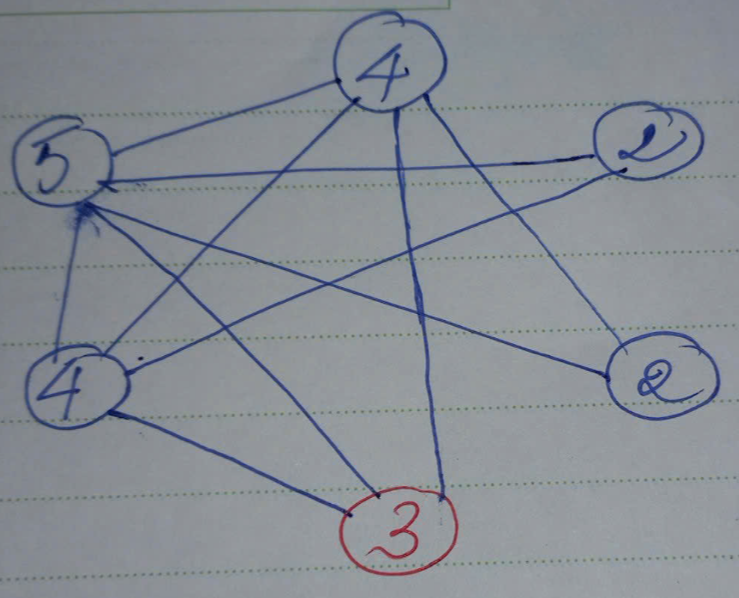
\includegraphics[scale=0.35]{Figures/A_03_01_02.png}
\end{center}

\textbf{Trường hợp 3. }Bậc của đỉnh còn lại bằng 1. Khi đó, dãy bậc của đồ thị là $5,\,4,\,4,\,2,\,2,\,1$, là một dãy graphic. Theo thuật toán Havel-Hakimi, dãy $3,\,3,\,1,\,1,\,0$ và $2,\,0,\,0,\,0$ cũng là các dãy graphic. Tuy nhiên, hiển nhiên không tồn tại đồ thị đơn 4 đỉnh có dãy bậc $2,\,0,\,0,\,0$. Do đó bậc của đỉnh còn lại của đồ thị đã cho không thể bằng 1.

Như vậy bậc của đỉnh còn lại của đồ thị đã cho chỉ có thể là 3. 

\begin{tcolorbox}[breakable]
    \begin{baitoan}[\parencite{shahriari2021invitation}, P10.1.15, p. 368]\label{pb:w02:06}
        Liệu có tồn tại đồ thị đơn mà các đỉnh có bậc là các số nguyên phân biệt? Câu hỏi tương tự cho đồ thị đa.
    \end{baitoan}
\end{tcolorbox}

\textbf{Lời giải. }Giả sử tồn tại đồ thị đơn có $n$ đỉnh thỏa mãn các đỉnh có bậc là các số nguyên phân biệt, ký hiệu các đỉnh là $v_0,\,v_1,\,\ldots,\,v_{n-1}$. Khi đó bậc của mỗi đỉnh sẽ thuộc tập $\{0,\,1,\,2,\,\ldots,\,n-1\}$. Tập hợp này có $n$ phần tử, mà mỗi đỉnh trong đồ thị phải có bậc là các số nguyên phân biệt nên $\deg(v_i) = i$ với mọi $i$. Khi đó, đỉnh $v_{n-1}$ có bậc là $n-1$ nên sẽ nối với tất cả các đỉnh còn lại, đỉnh $v_0$ có bậc là 0 nên không nối với đỉnh nào, điều này mâu thuẫn. Như vậy không tồn tại đồ thị đơn thỏa mãn đề.

Đối với đồ thị đa, câu trả lời là khẳng định. Thật vậy, chẳng hạn xét đồ thị đa có 4 đỉnh như hình bên dưới, khi đó bậc của các đỉnh lần lượt là $1,\,2,\,3,\,4$. 

\begin{center}
    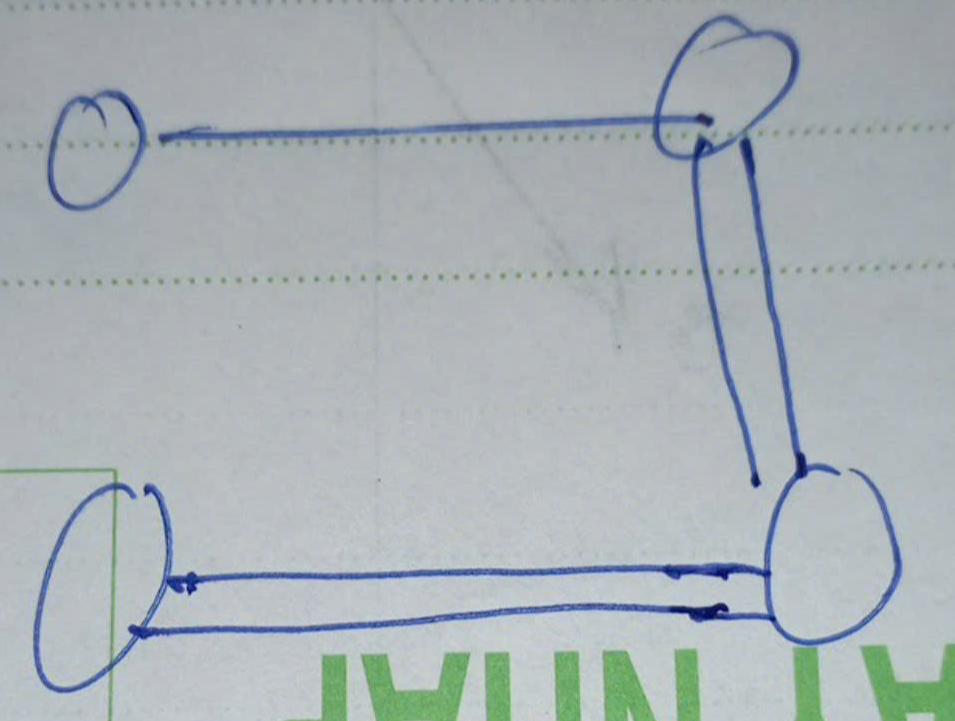
\includegraphics[scale=0.3]{Figures/A_03_01_01.png}
\end{center}

\begin{tcolorbox}[breakable]
    \begin{baitoan}[\parencite{shahriari2021invitation}, P10.1.16, p. 368]\label{pb:w02:05}
        Xét đồ thị đơn $G$ có 94 đỉnh. Giả sử rằng tất cả các đỉnh của $G$ đều có bậc là số lẻ. Chứng minh rằng tồn tại ít nhất ba đỉnh có cùng bậc.
    \end{baitoan}
\end{tcolorbox}

\textbf{Lời giải. }Ta sẽ chứng minh cho trường hợp tổng quát với đồ thị $G$ có $2n$ đỉnh. Do $G$ là đồ thị đơn nên bậc của mỗi đỉnh sẽ thuộc tập $\{0,\,1,\,2,\,\ldots,\,2n-1\}$. Mặt khác, tất cả các đỉnh của $G$ đều có bậc lẻ nên bậc của mỗi đỉnh sẽ thuộc tập $U = \{1,\,3,\,5,\,\ldots,\,2n-1\}$. Giả sử chỉ có tối đa hai đỉnh có cùng bậc, thì khi đó mỗi phần tử trong $U$ sẽ có đúng 2 đỉnh nhận làm bậc, suy ra dãy bậc của đồ thị $G$ sẽ là $$2n-1,\,2n-1,\,2n-3,\,2n-3,\,\ldots,\,3,\,3,\,1,\,1.$$

Áp dụng thuật toán Havel-Hakimi, khi đó dãy $$2n-2,\,2n-4,\,2n-4,\,\ldots,\,2,\,2,\,0,\,0$$ phải là một dãy graphic. Tuy nhiên, không tồn tại đồ thị đơn có $2n-1$ đỉnh thỏa mãn tồn tại một đỉnh có bậc $2n-2$ và một đỉnh có bậc $0$. Như vậy, có ít nhất ba đỉnh trong $G$ có cùng bậc.

\begin{tcolorbox}[breakable]
    \begin{baitoan}\label{pb:w08:01}
        Cho $G = (V,\,E)$ là đồ thị tổng quát với $d_1,\,\ldots,\,d_p\in\mathbb{N}$ là bậc của các đỉnh. Chứng minh: Bậc cao nhất $d_{\max}\coloneqq\max_{1\le i\le p} d_i$ thỏa $d_{\max}\ge\dfrac{2|E|}{|V|}$.
    \end{baitoan}
\end{tcolorbox}

\textbf{Lời giải. }Theo định lý Euler thì $d_1 + d_2 + \cdots + d_p = 2|E|$. Vì $d_{\max} \geq d_i,\,\forall i$ nên $2|E| \leq p\cdot d_{\max} = |V| \cdot d_{\max}$. Suy ra $d_{\max} \geq \dfrac{2|E|}{|V|}$.


% \begin{tcolorbox}[breakable]
%     \begin{baitoan}[\cite{shahriari2021invitation}, P10.1.17, p. 368]\label{pb:w08:02}
%         Giả sử rằng $a_1\ge a_2\ge\cdots a_n$ là một dãy graphic. Chứng minh rằng với mọi $1 \leq k \leq n$ thì 
%         \begin{equation*}
%             \sum_{i=1}^k a_i\le k(k - 1) + \sum_{i=k+1}^n \min\{k,\,a_i\}.
%         \end{equation*}
%     \end{baitoan}
% \end{tcolorbox}

% \textbf{Lời giải. }

% \begin{tcolorbox}[breakable]
%     \begin{baitoan}[\cite{shahriari2021invitation}, P10.1.18, p. 368]\label{pb:w08:03}
%         Xét $p,\,t\in\mathbb{N}^\star$ với $2\le t < p$. Giả sử rằng $a_1\ge a_2\ge\cdots\ge a_{t-1} > a_t\ge\cdots\ge a_{p-1} > a_p$ là dãy bậc của một đồ thị đơn. Chứng minh rằng $a_1\ge a_2\ge\cdots\ge a_{t-1}\ge a_t + 1\ge\cdots\ge a_{p-1}\ge a_p + 1$ cũng là dãy bậc của một đồ thị đơn.
%     \end{baitoan}
% \end{tcolorbox}

% \textbf{Lời giải. }

% \begin{tcolorbox}[breakable]
%     \begin{baitoan}[\cite{shahriari2021invitation}, P10.1.19, pp. 368--369]\label{pb:w08:04}
%         Tồn tại hay không đồ thị đơn với $48$ đỉnh, trong đó tập hợp bậc của các đỉnh là $\{4,\,7,\,47\}$? Tổng quát, xét $S = \{a_1,\,\ldots,\,a_n\}$ là tập hợp khác rỗng gồm $n$ số nguyên dương với $a_1 < a_2 < \cdots < a_n$. Chứng minh rằng tồn tại đồ thị đơn $G$ với $a_n + 1$ đỉnh, trong đó tập hợp bậc của các đỉnh chính là $S$. 
%     \end{baitoan}
% \end{tcolorbox}

% \textbf{Lời giải. }